\section{レポート課題2}
\subsection{課題1}
ジスティク写像で $r = 1.50, r = 2.60, r = 3.20, r = 3.50, r = 3.86, r = 3.90$ として、初期値$x_0$ を $0$ から $1$ まで $0.001$ きざみで変化させたときの、$x_{200}$ の値がどうなっているかグラフ化せよ。また、$x_n$ が $150 < n < 200$ の場合もグラフ化せよ。出力形式は授業資料を参照すること。\\
画像:\\
\begin{figure}[htbp]
  \begin{tabular}{cc}
    \begin{minipage}[t]{0.45\hsize}
      \centering
      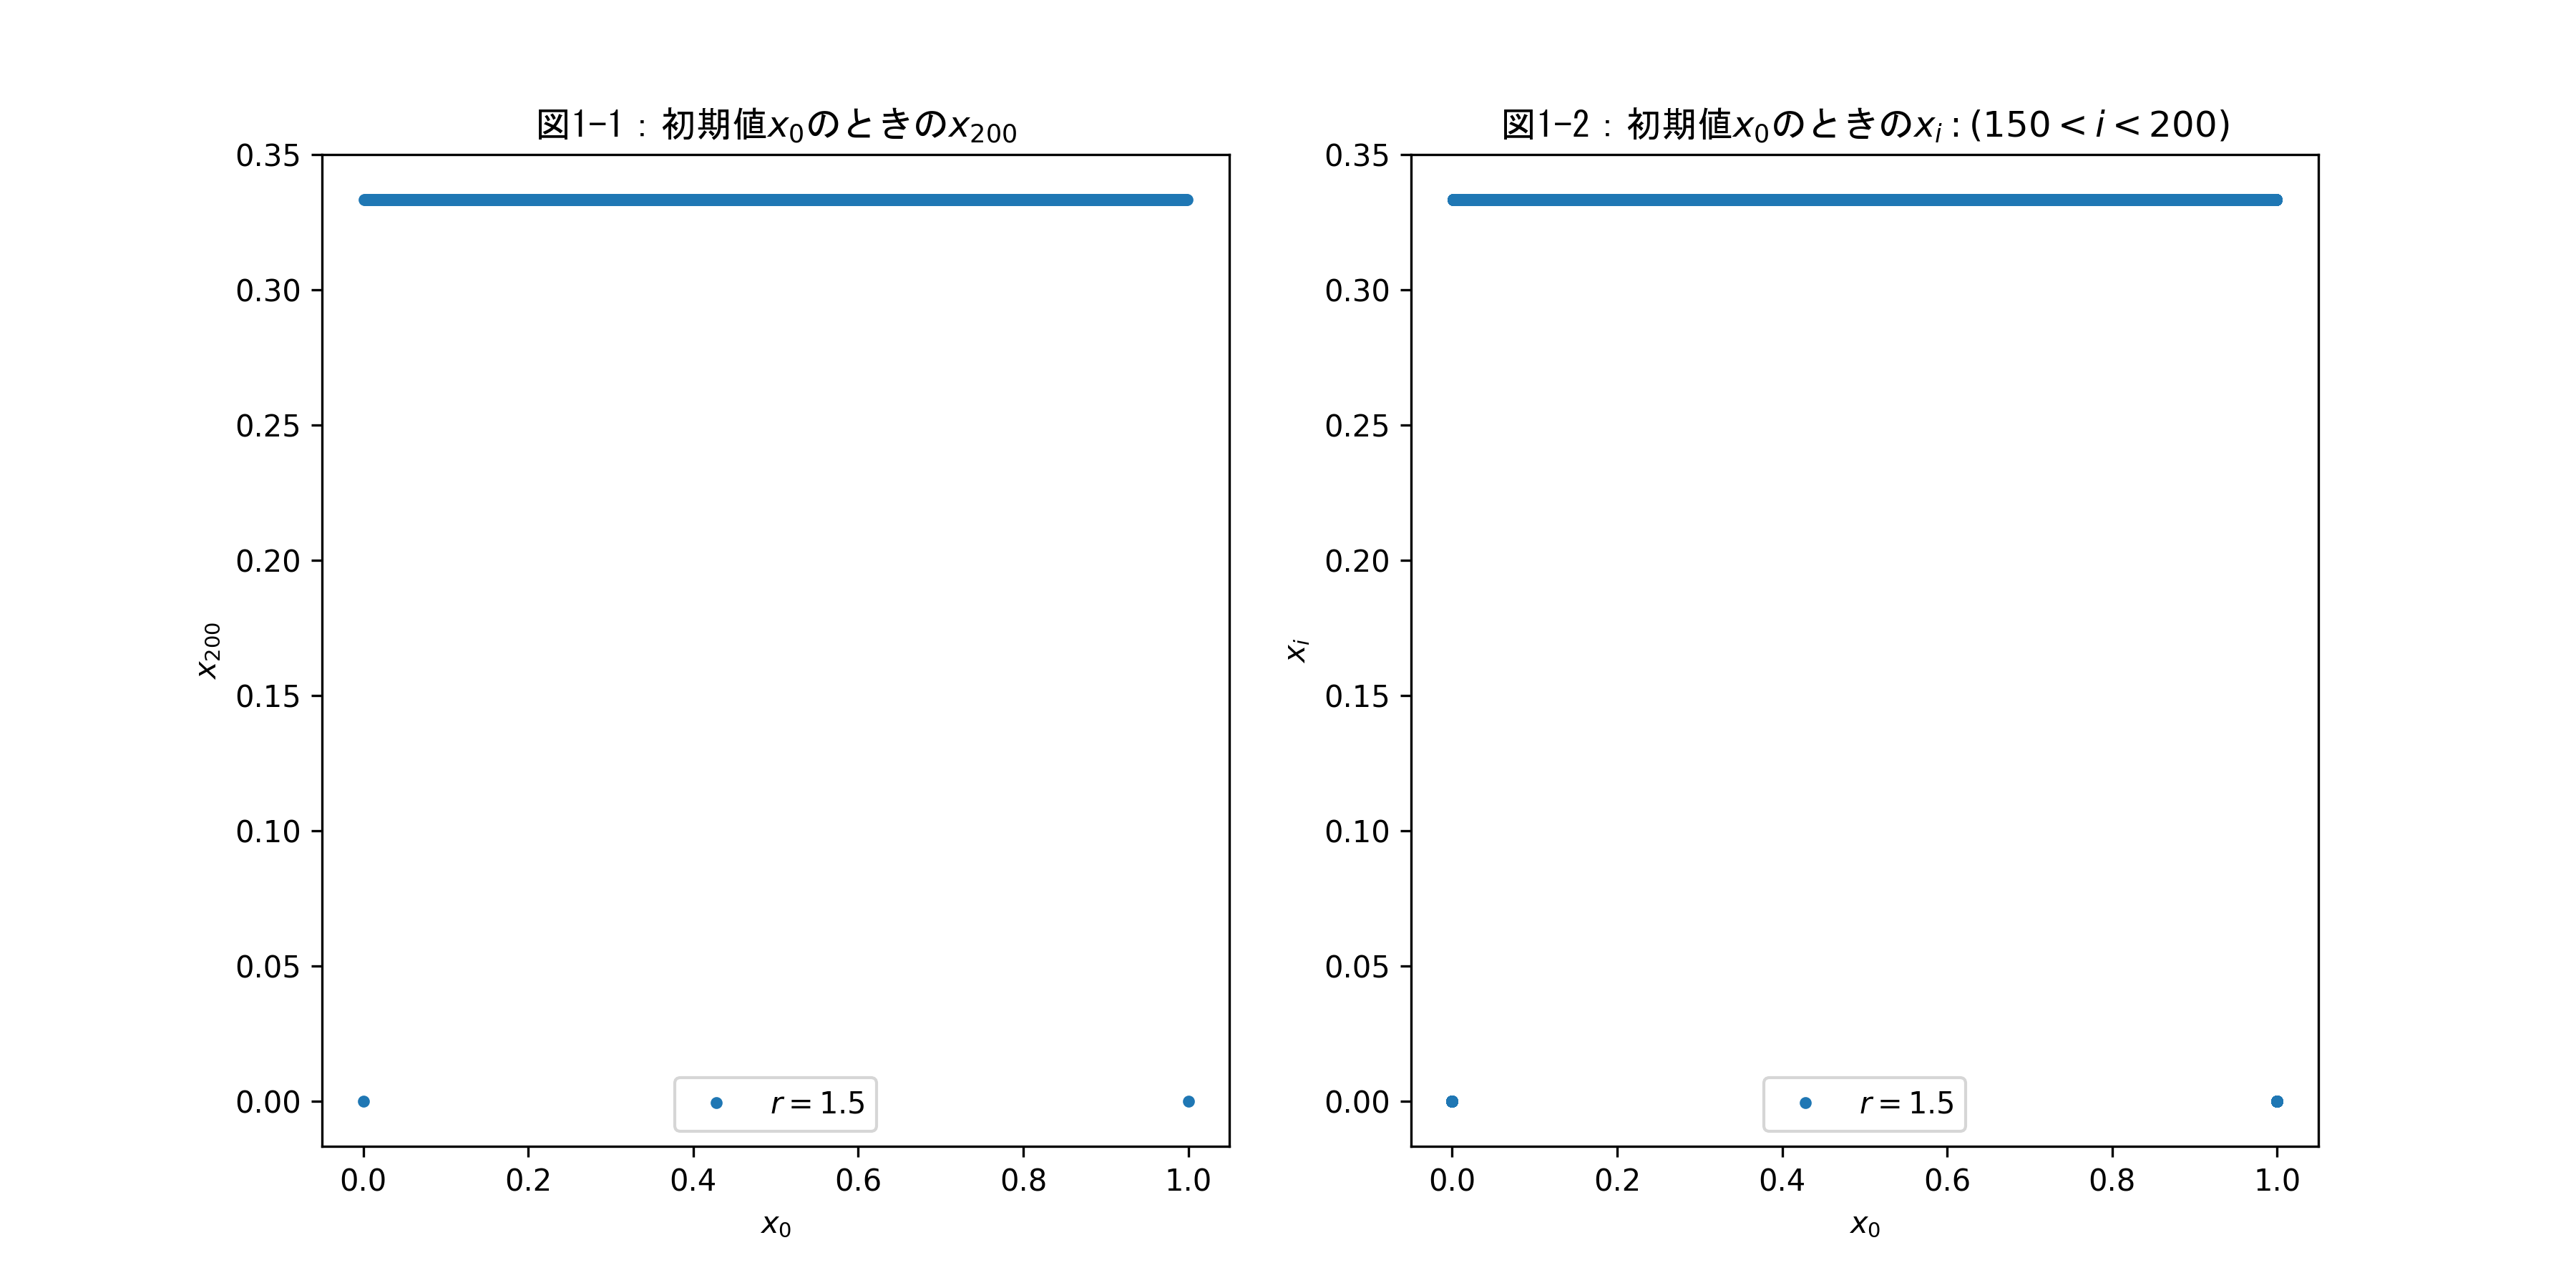
\includegraphics[keepaspectratio, scale=0.25]{images/Problem2/ctest3_1.png}
    \end{minipage} &
    \begin{minipage}[t]{0.45\hsize}
      \centering
      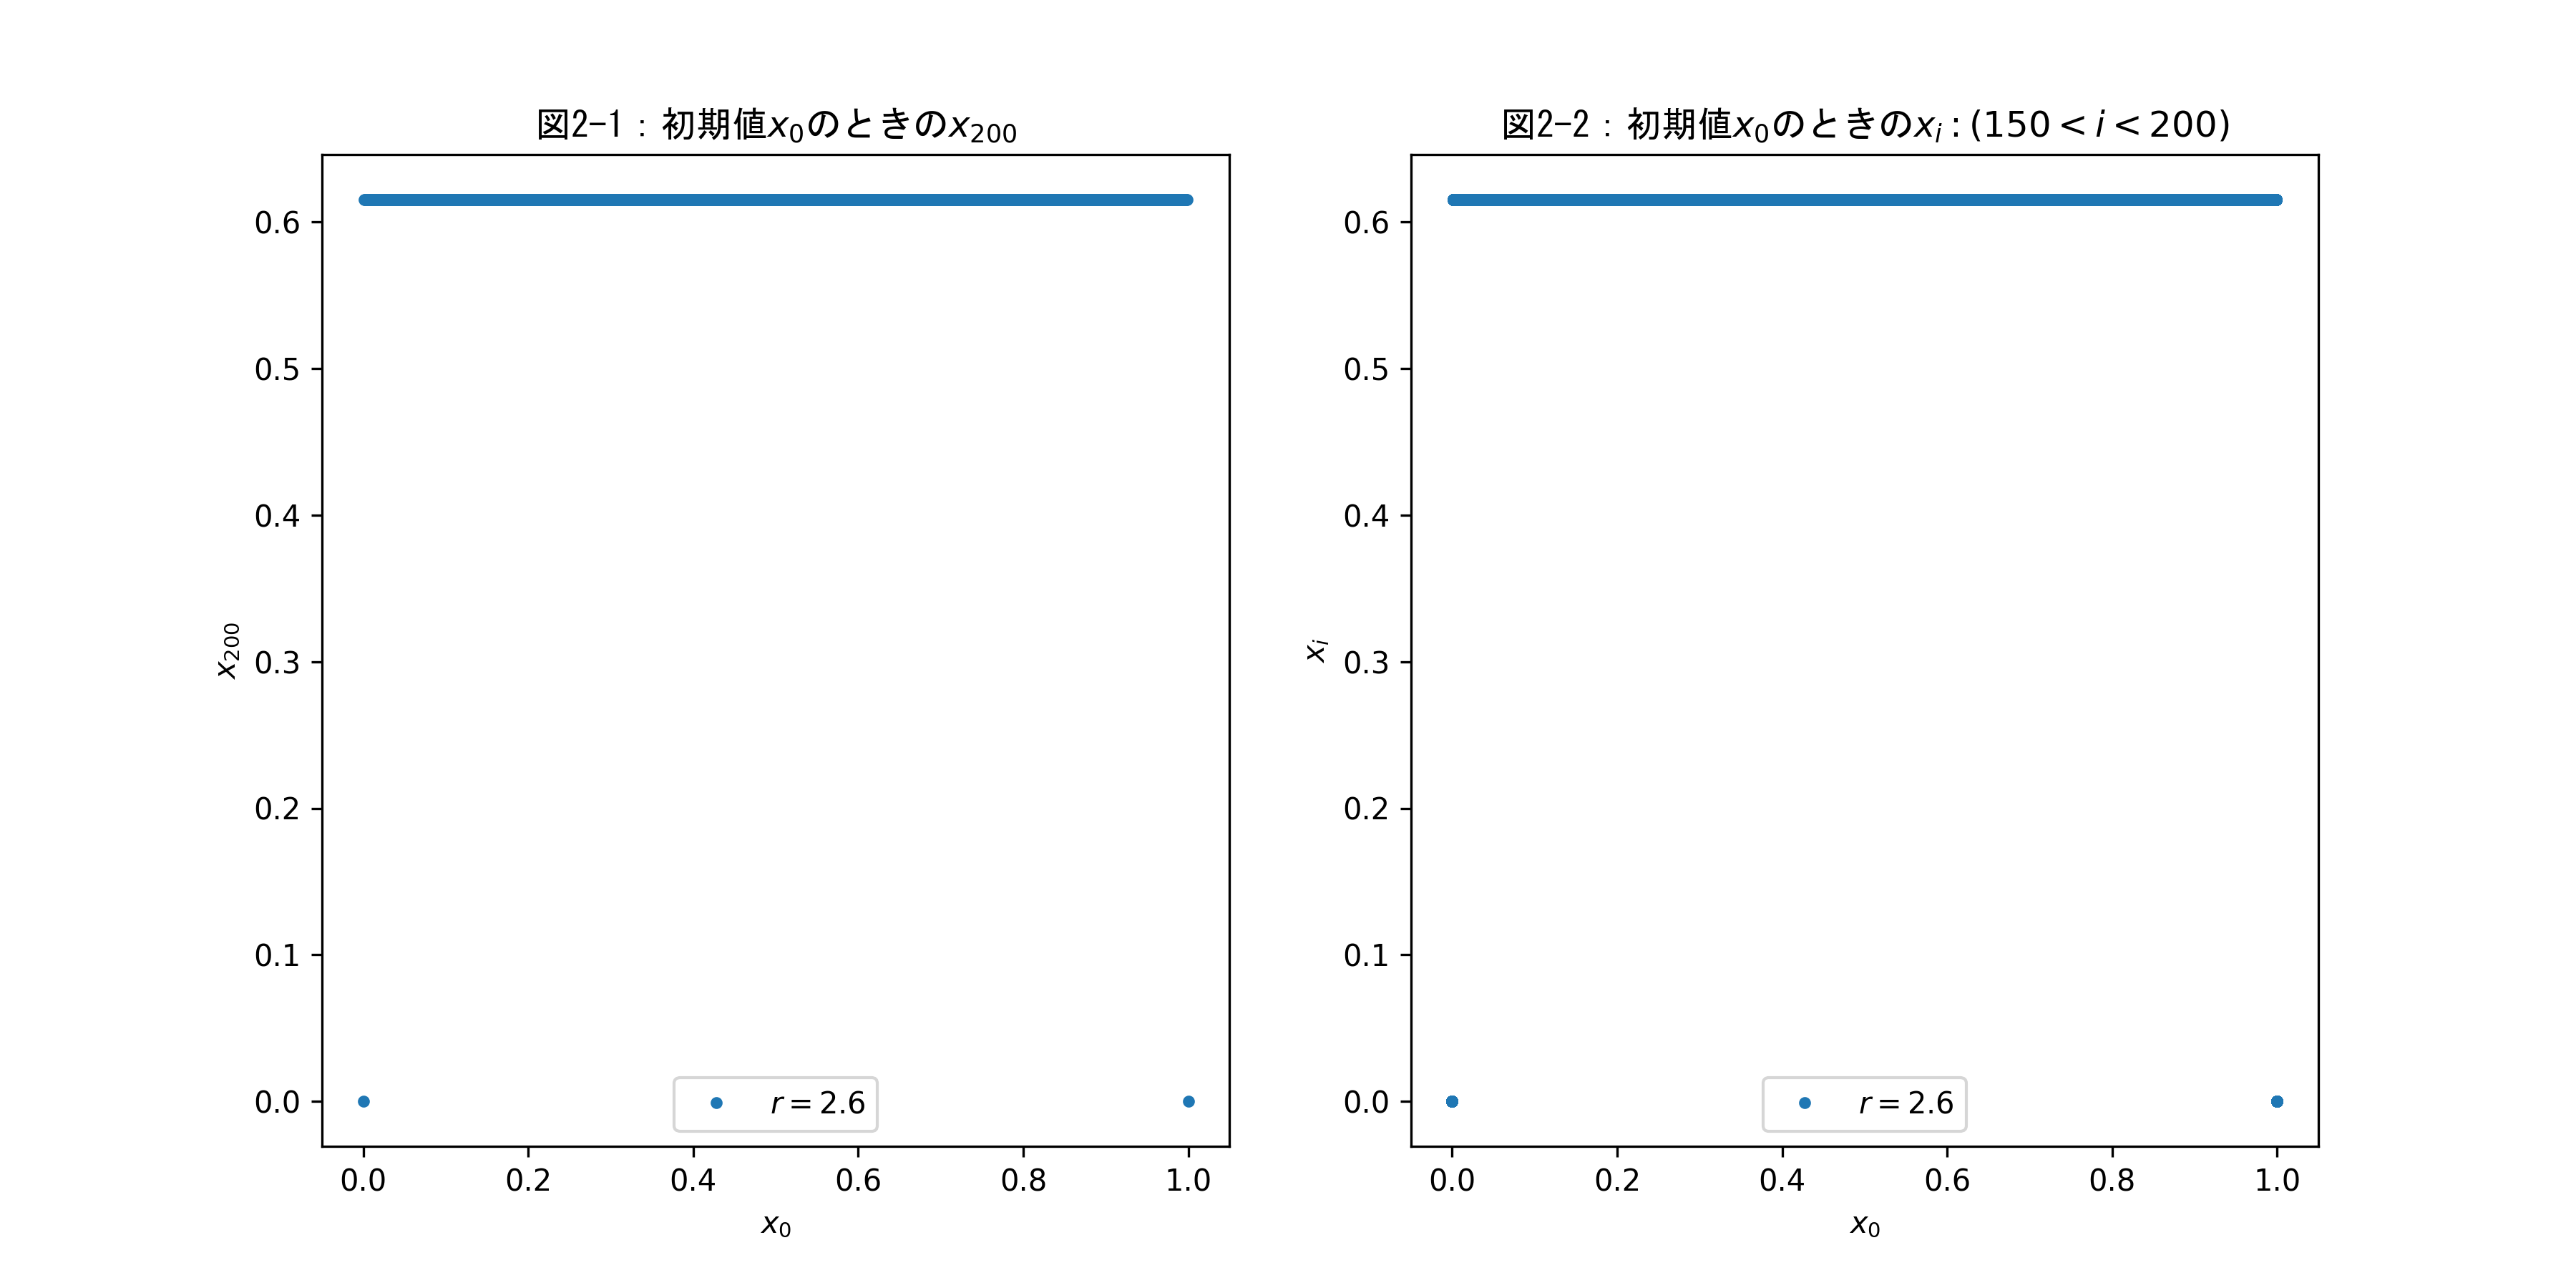
\includegraphics[keepaspectratio, scale=0.25]{images/Problem2/ctest3_2.png}
    \end{minipage} \\

    \begin{minipage}[t]{0.45\hsize}
      \centering
      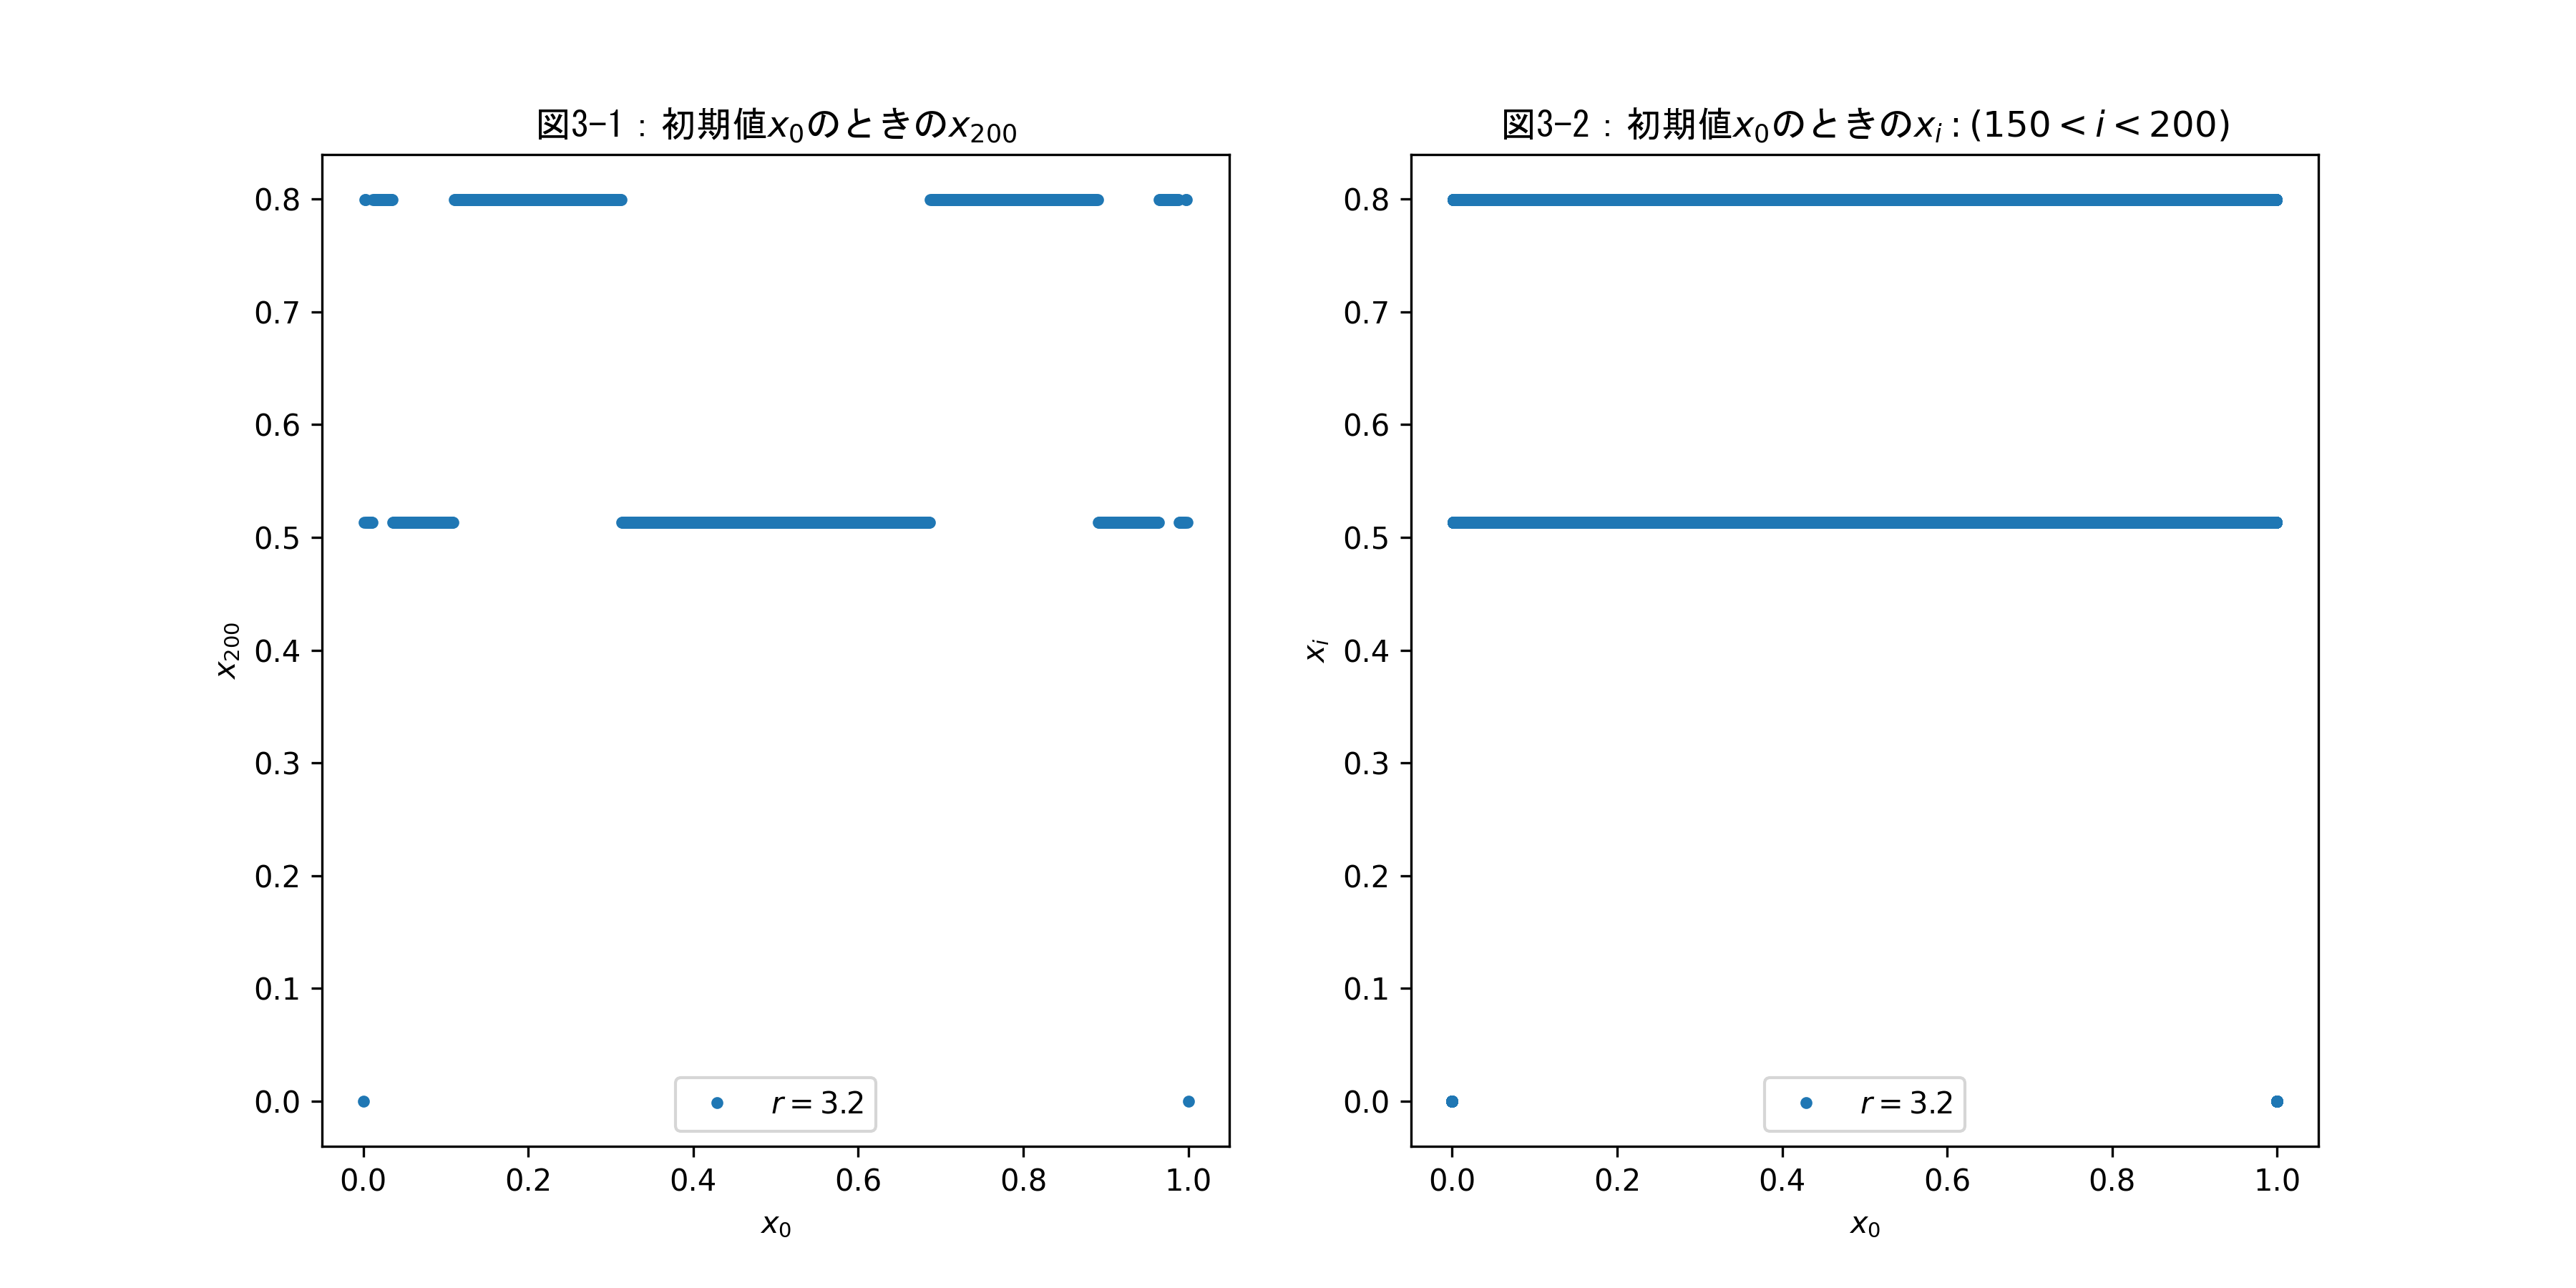
\includegraphics[keepaspectratio, scale=0.25]{images/Problem2/ctest3_3.png}
    \end{minipage} &
    \begin{minipage}[t]{0.45\hsize}
      \centering
      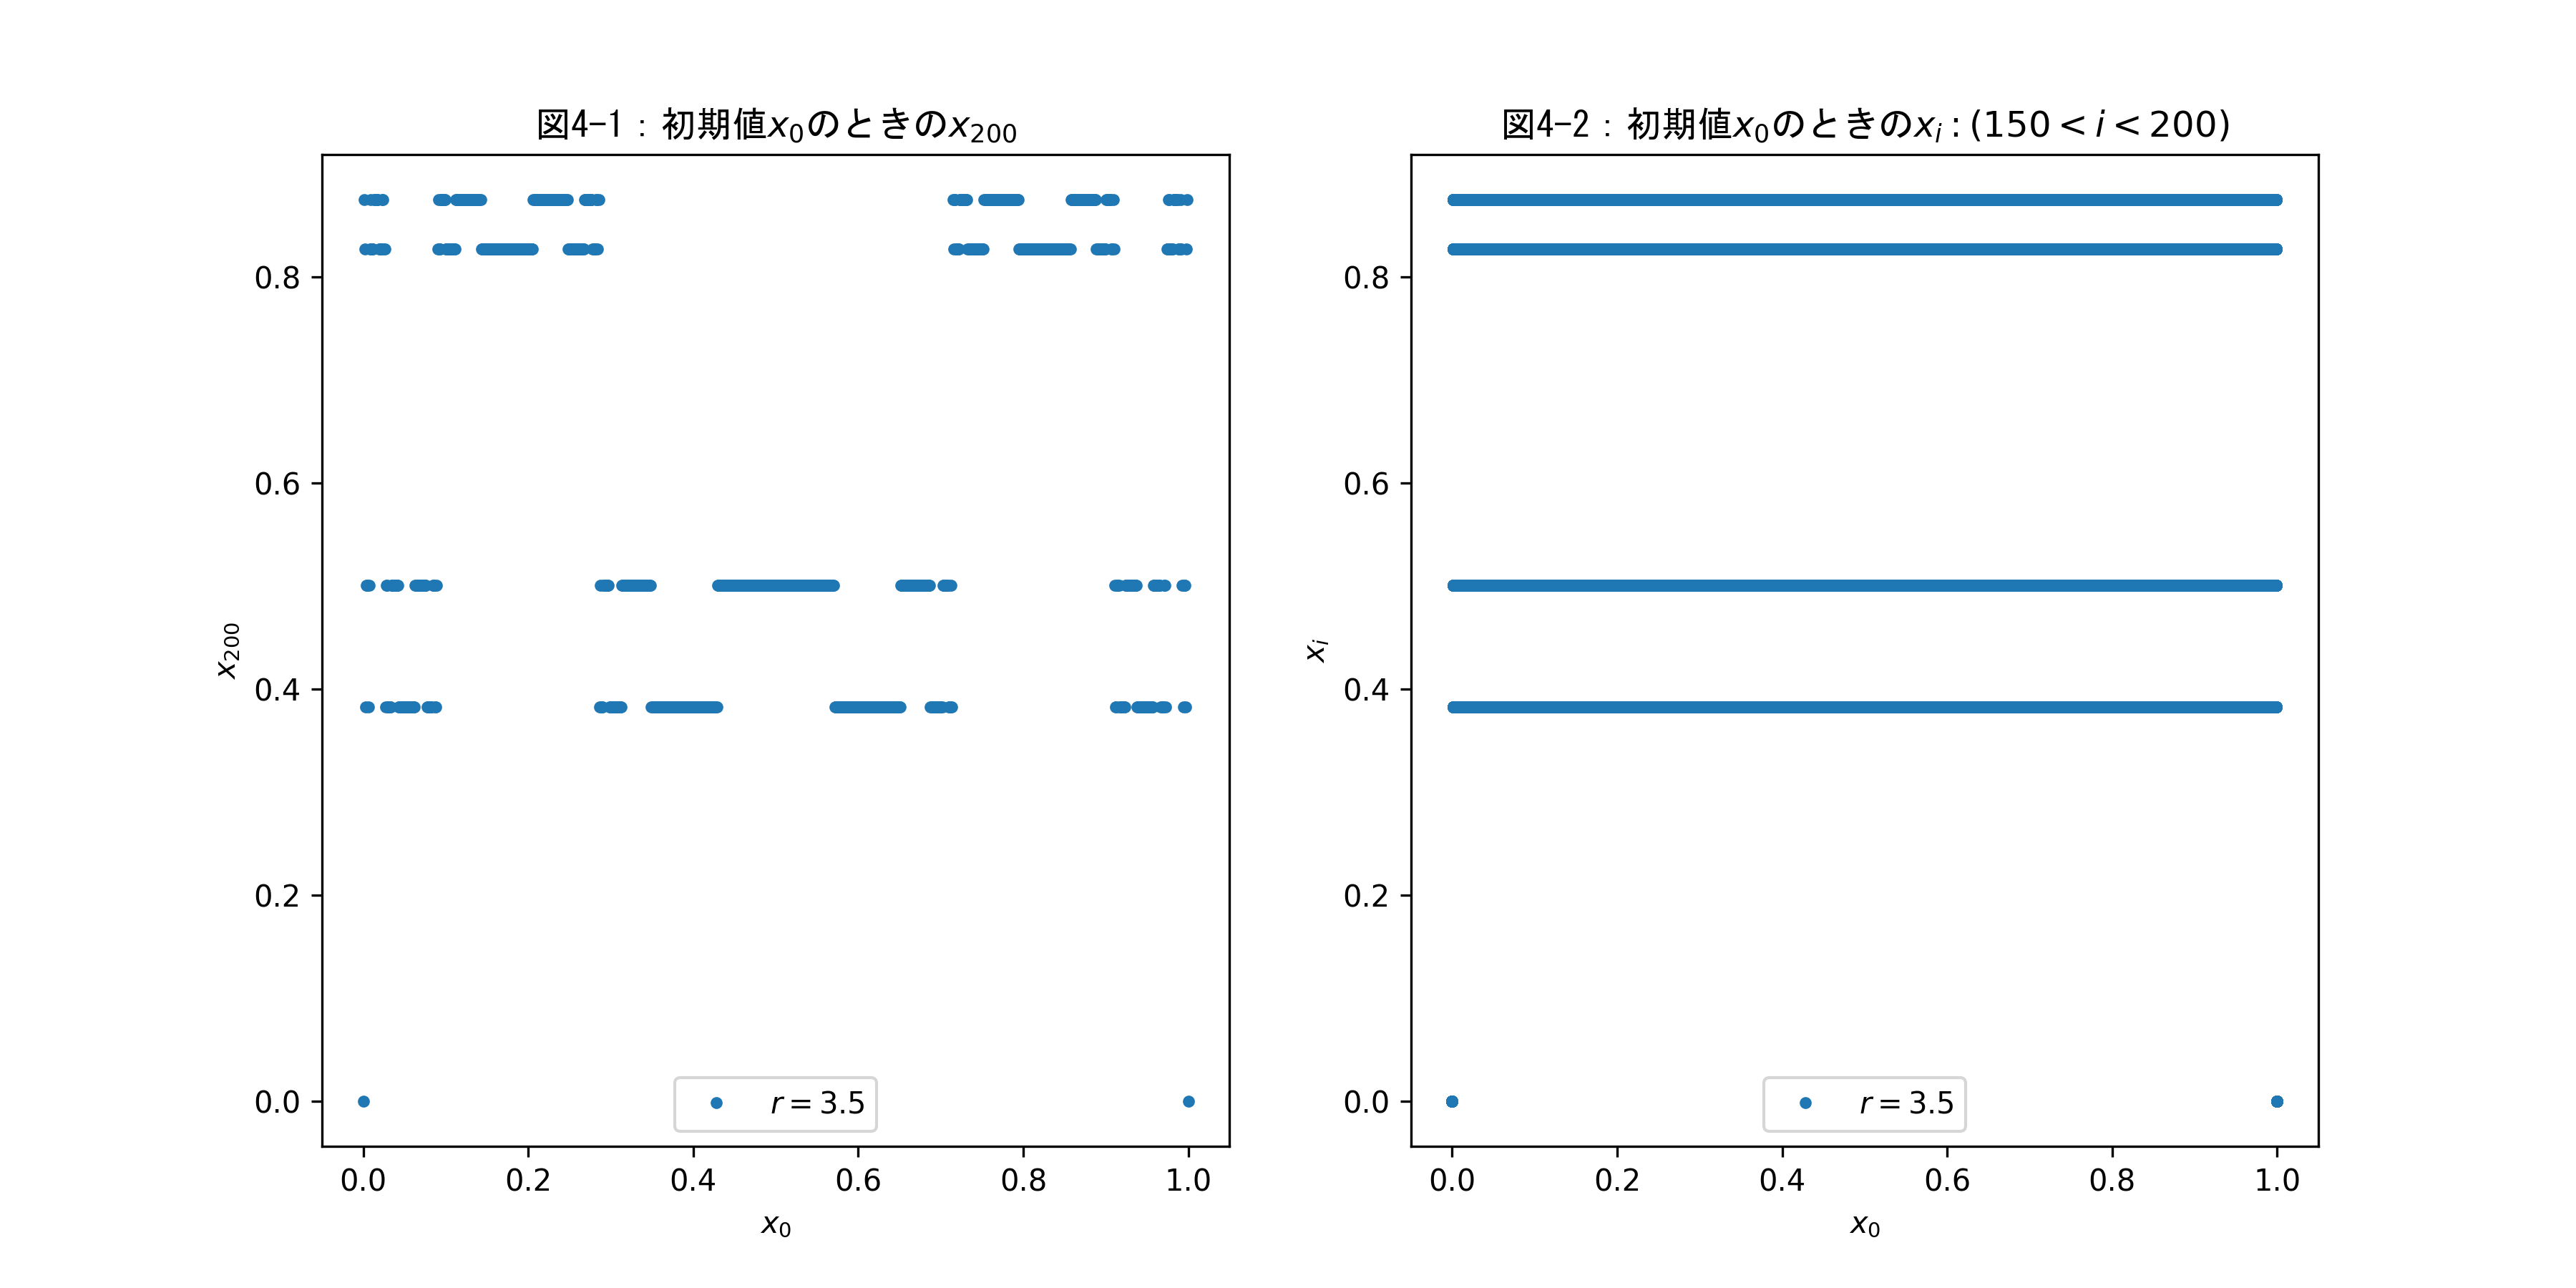
\includegraphics[keepaspectratio, scale=0.25]{images/Problem2/ctest3_4.png}
    \end{minipage} \\

    \begin{minipage}[t]{0.45\hsize}
      \centering
      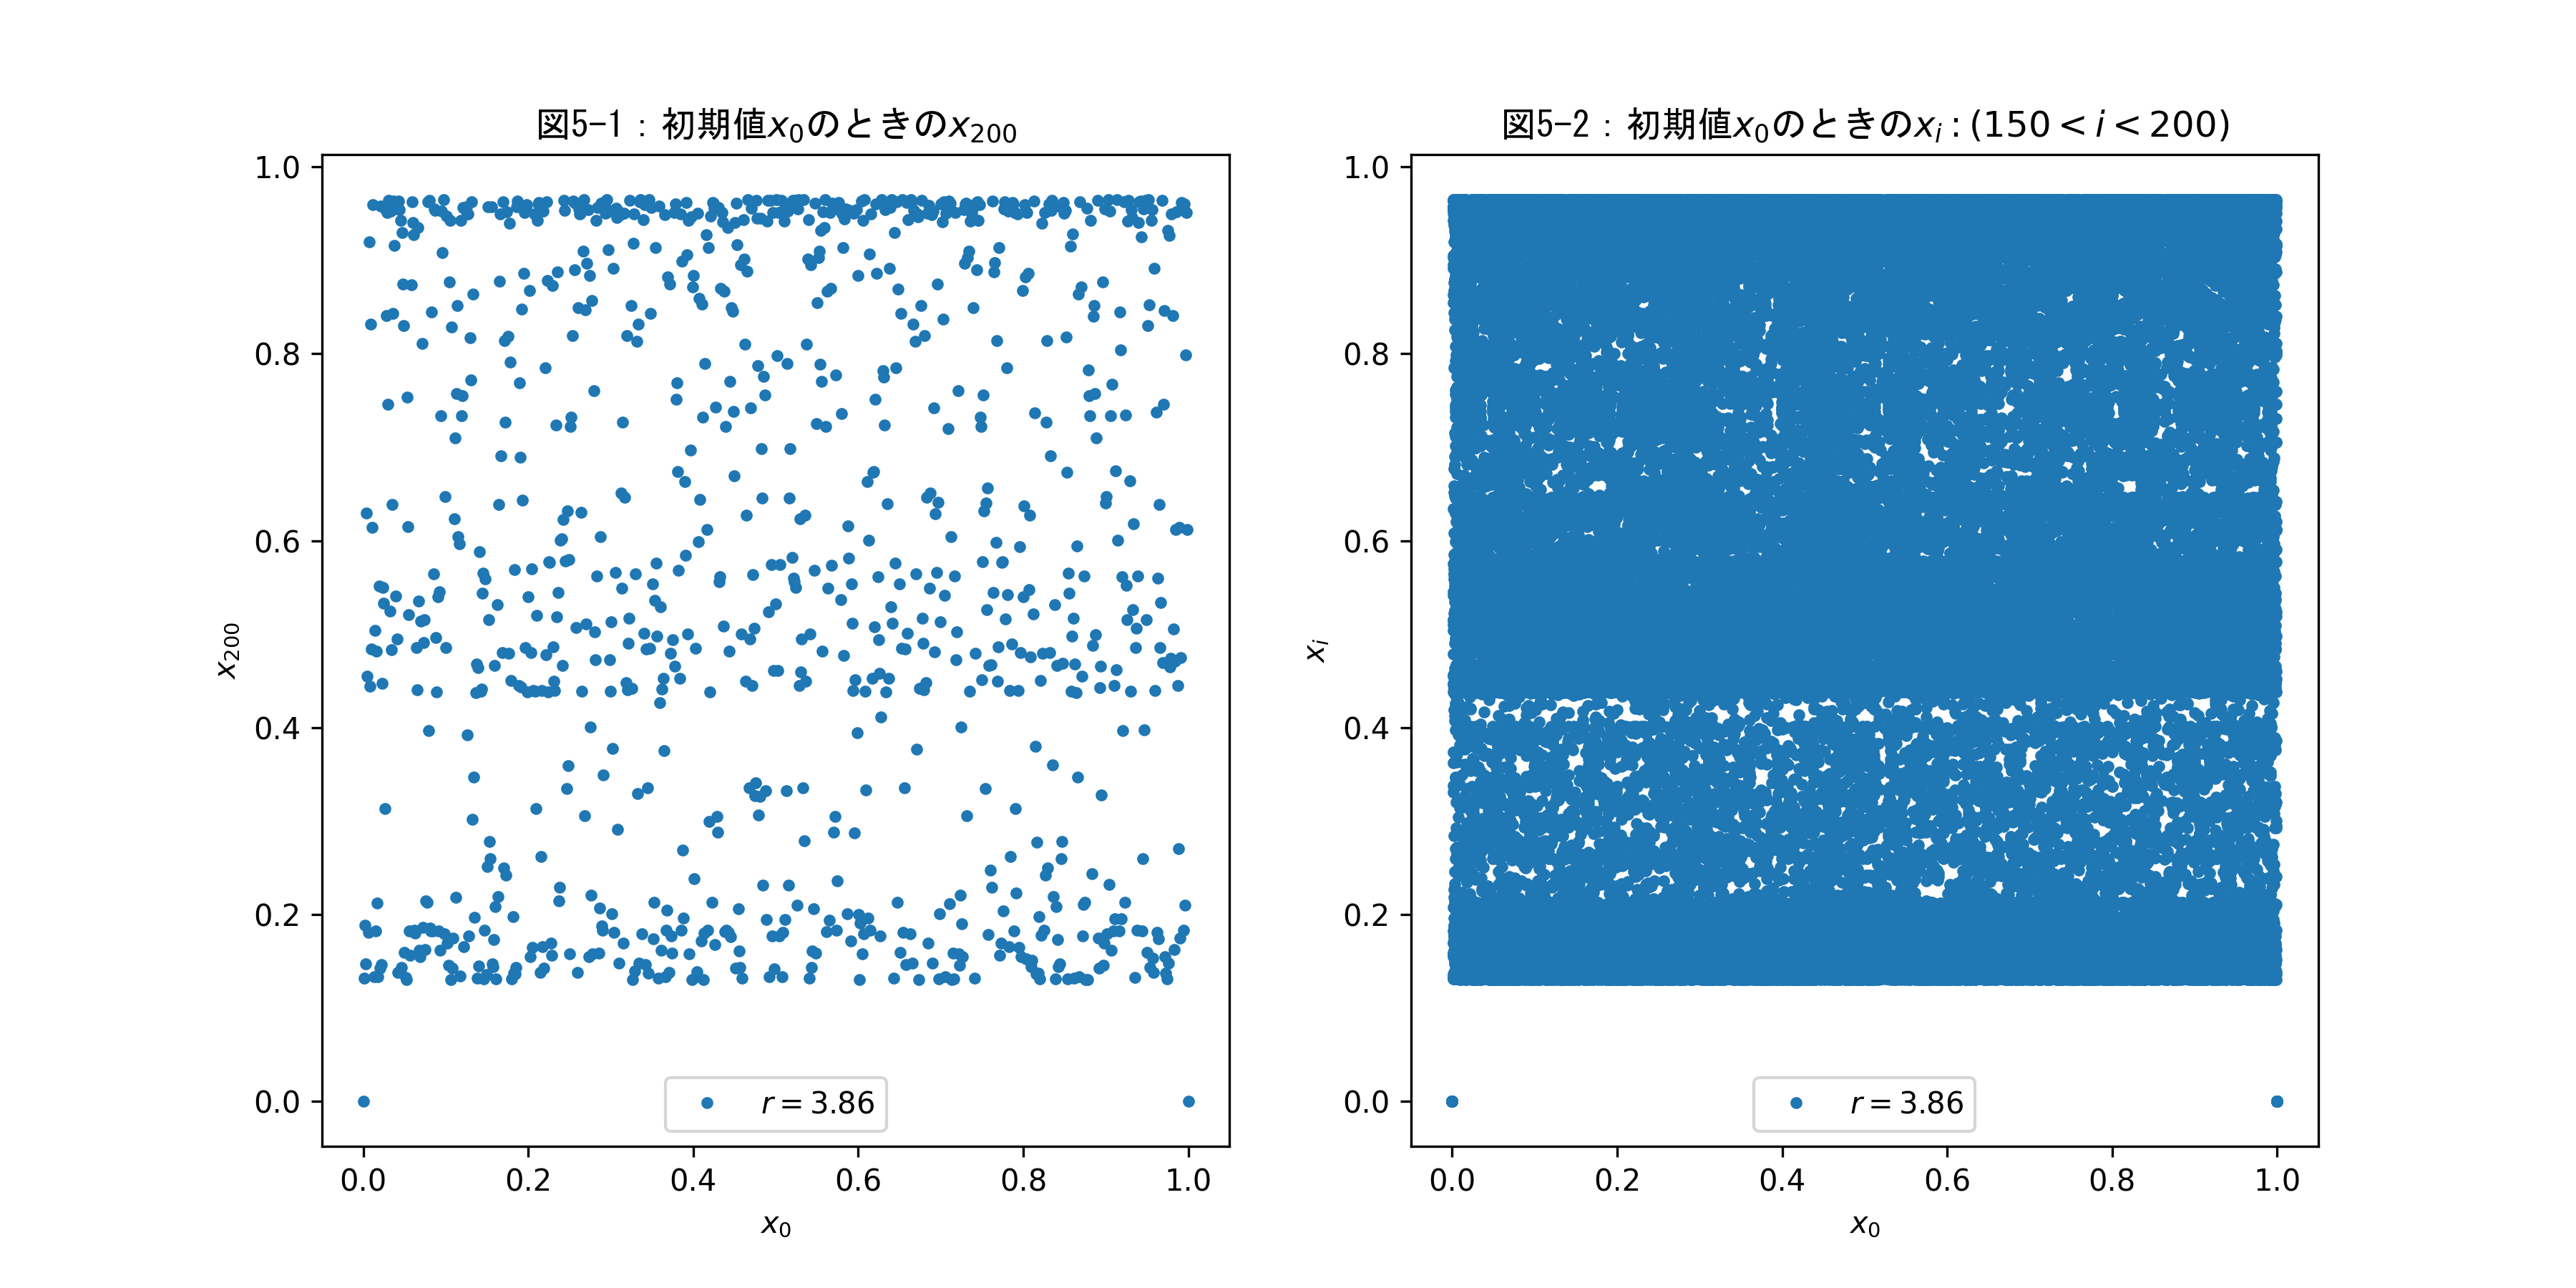
\includegraphics[keepaspectratio, scale=0.25]{images/Problem2/ctest3_5.png}
    \end{minipage} &
    \begin{minipage}[t]{0.45\hsize}
      \centering
      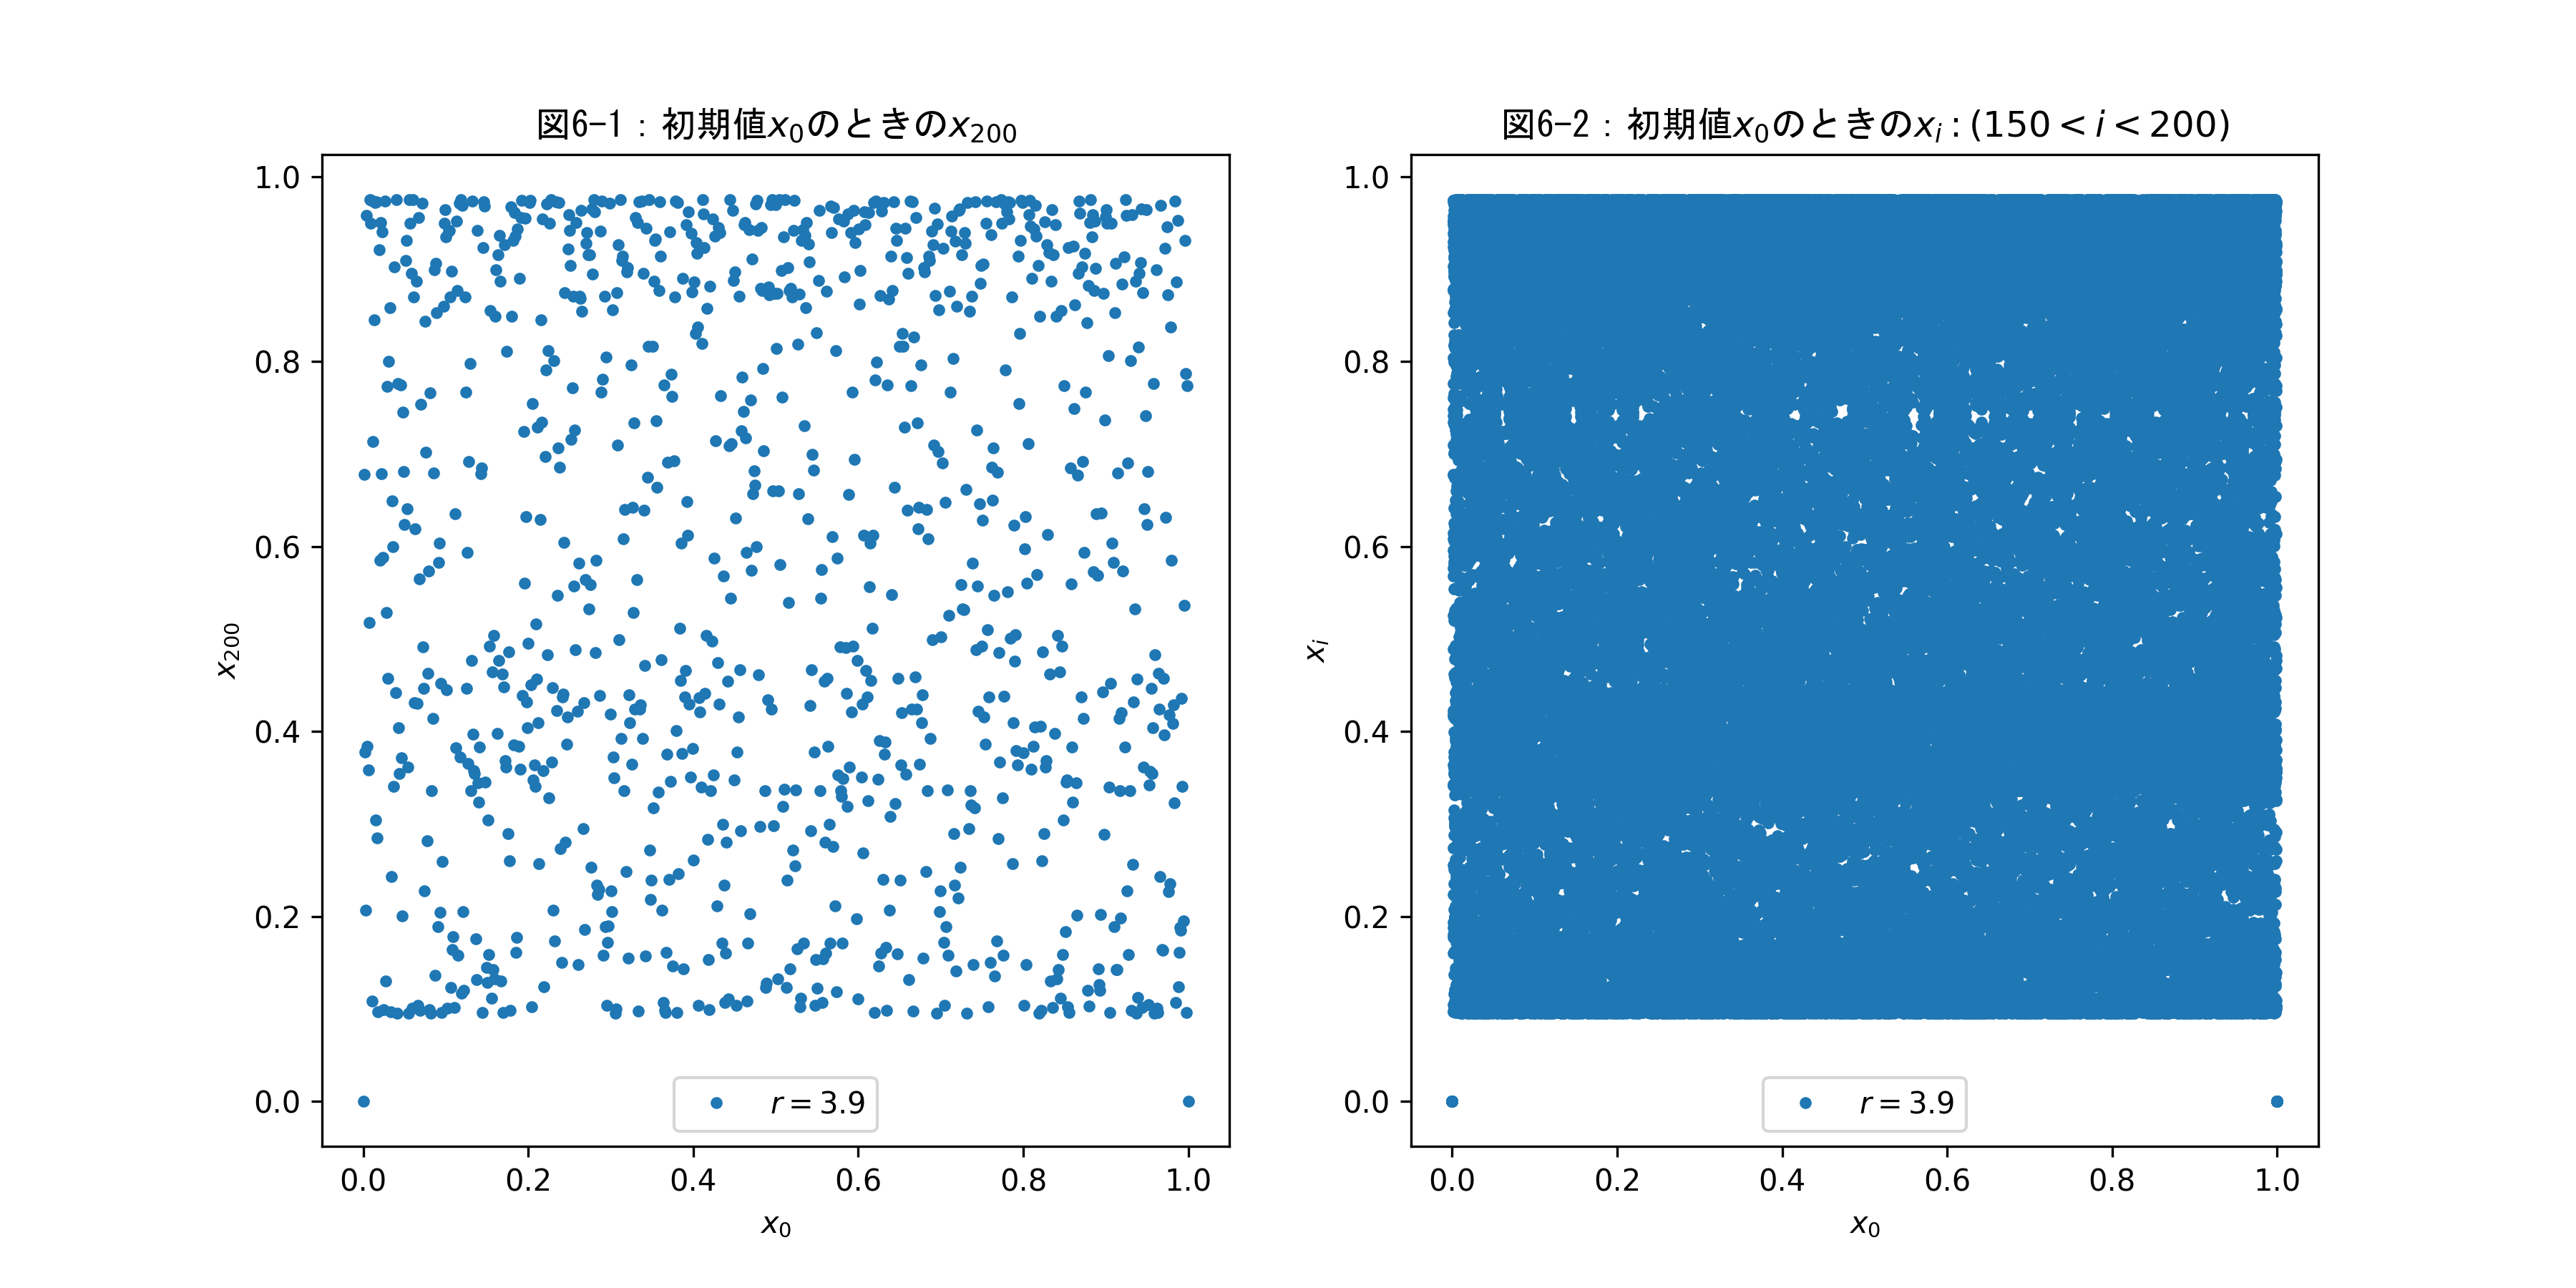
\includegraphics[keepaspectratio, scale=0.25]{images/Problem2/ctest3_6.png}
    \end{minipage}
  \end{tabular}
\end{figure}


結果:\\
$r = 1.50, r = 2.60$ のときは、$x_{200}$, $x_n (150 < n < 200)$ のどちらも値は一つに定まる。 $r = 3.20$ のときは、 $x_{200}$, $x_n (150 < n < 200)$ は2通りの値のどちらかに定まることが読み取れる。また、 $r = 3.50$ のときは、 $x_{200}$, $x_n (150 < n < 200)$ は4通りの値のいづれかに定まる。$r = 3.86, r = 3.90$ のときは、 $x_{200}$, $x_n (150 < n < 200)$ のどちらもある値に定まることはなく、不規則な値を取り続けている。\\\\

考察:\\
これらの結果から、 $r = 3.86, r = 3.90$ のときは初期値 $x_0$ の小さい変化によって$x_{200}$ と $x_n (150 < n < 200)$ が大きく変化することが考察できる。

\subsection{課題2}
課題1で得られた結果から初期値鋭敏性を説明せよ。\\
課題1で得られた結果から考察した際に、「$r = 3.86, r = 3.90$ のときは初期値 $x_0$ の小さい変化によって$x_{200}$ と $x_n (150 < n < 200)$ が大きく変化することが考察できる。」と書いたが、このように初期値の小さい変化である数 $n$ のときの $x_n$ の値が大きく変化することを初期値鋭敏性という。

\subsection{ソースコード}
\begin{lstlisting}[caption=week2.py]
  import numpy as np
  import matplotlib
  from matplotlib import pyplot as plt
  # 日本語フォント用(Linux)
  matplotlib.rc('font', family='Noto Sans CJK JP')
  '''
  # 日本語フォント用(Windows)
  matplotlib.rc('font', family='MS Gothic')
  '''
  
  class Task2():
      def __init__(self, r: float, file_name: str, index: int) -> None:
          self.r = r
          self.file_name = file_name
          self.index = index
          self.x = np.linspace(0, 1, 1000)
          fig = plt.figure(figsize=(12, 6))
          self.ax1 = fig.add_subplot(1, 2, 1)
          self.ax2 = fig.add_subplot(1, 2, 2)
  
      def code_problem1(self) -> None:
          "課題1について処理をしている関数"
          ax1_array = []
          for i in self.x:
              num = i
              for j in range(200):
                  num = self.r * num * (1 - num)
              ax1_array.append(num)
          self.ax1.set_xlabel('$x_0$')
          ylabel = '$x_{200}$'
          self.ax1.set_ylabel(ylabel)
          self.ax1.set_title('図{0}-1:初期値'.format(self.index) +
                             '$x_0$のときの' + ylabel)
          self.ax1.plot(self.x, ax1_array, marker='.',
                        linestyle='None', label='$r = $' + str(self.r))
          self.ax1.legend(loc='best')
  
      def code_problem2(self) -> None:
          "課題2について処理をしている関数"
          ax2_array = []
          x_array = []
          for i in self.x:
              num = i
              for j in range(200):
                  num = self.r * num * (1 - num)
                  if 150 <= j:
                      ax2_array.append(num)
                      x_array.append(i)
          self.ax2.set_xlabel('$x_0$')
          self.ax2.set_ylabel('$x_{i}$')
          self.ax2.set_title(
              '図{0}-2:初期値$x_0$のときの$x_i : (150 < i < 200)$'.format(self.index))
          self.ax2.plot(x_array, ax2_array, marker='.',
                        linestyle='None', label='$r = $' + str(self.r))
          self.ax2.legend(loc='best')
  
      def show_graph(self) -> None:
          file_path = '複雑系科学演習/Week2/images/'
          plt.savefig(file_path + self.file_name, dpi=300)
          # plt.show()
  
  
  r = [1.50, 2.60, 3.20, 3.50, 3.86, 3.90]
  for i in range(len(r)):
      demo = Task2(r[i], 'task2_{}'.format(i + 1), i + 1)
      demo.code_problem1()
      demo.code_problem2()
      demo.show_graph()
\end{lstlisting}